\chapter{Rezultate obținute}

Acest capitol prezintă rezultatele obținute pe cele trei sisteme analizate, CockroachDB, TiDB și Citus, în patru configurații descrise mai devreme de cluster cu 3, 5, 10 și 20 de noduri.

Cele 22 de interogări au fost împărțite în patru grupe, definite anterior, pe baza profilului dominant al interogării. Fiecare secțiune de grupă este structurată în jurul a patru grafice generate din datele prelucrate cu \texttt{pandas} și \texttt{matplotlib}. Anumite celule din grafice apar marcate „N/A”, aceste lipsuri nu reprezintă erori de măsurare, ci constatări arhitecturale documentate.

\section{Grupa 1 - Interogări dominate de scanări}

Prima grupă, definită anterior este formată din interogările Q1, Q6, Q14 și Q19, ale căror planuri de implementare în toate sistemele de baze de date sunt similare și sunt dominate de o scanare integrală sau filtrată a celei mai mari tabele din benchmark, \texttt{lineitem}. Q1 calculează o agregare pe două coloane de grupare cu un filtru pe \texttt{l\_shipdate}. Q6 selectează toată tabela \texttt{lineitem} și o reduce la un singur scalare pe baza mai multor predicate, Q14 efectuează un join selectiv cu \texttt{part} dar conform planurilor de execuție, timpul principal este petrecut în executarea scanării tabelului \texttt{lineitem} filtrat pe dată. Q19 efectuează o îmbinare similară cu cea din Q14 dar aplică predicate de filtrare complexe. În toate cele 4 interogări, costul dominant este parcurgerea celor aproximativ 180 de milioane de rânduri ale tabelei \texttt{lineitem} și aplicarea unor filtre relativ simple. Acest grup indică informații despre eficiența motorului de scanare și strategia de distribuire a tabelei voluminoase pe mai multe noduri.

\begin{figure}[H]
    \centering
    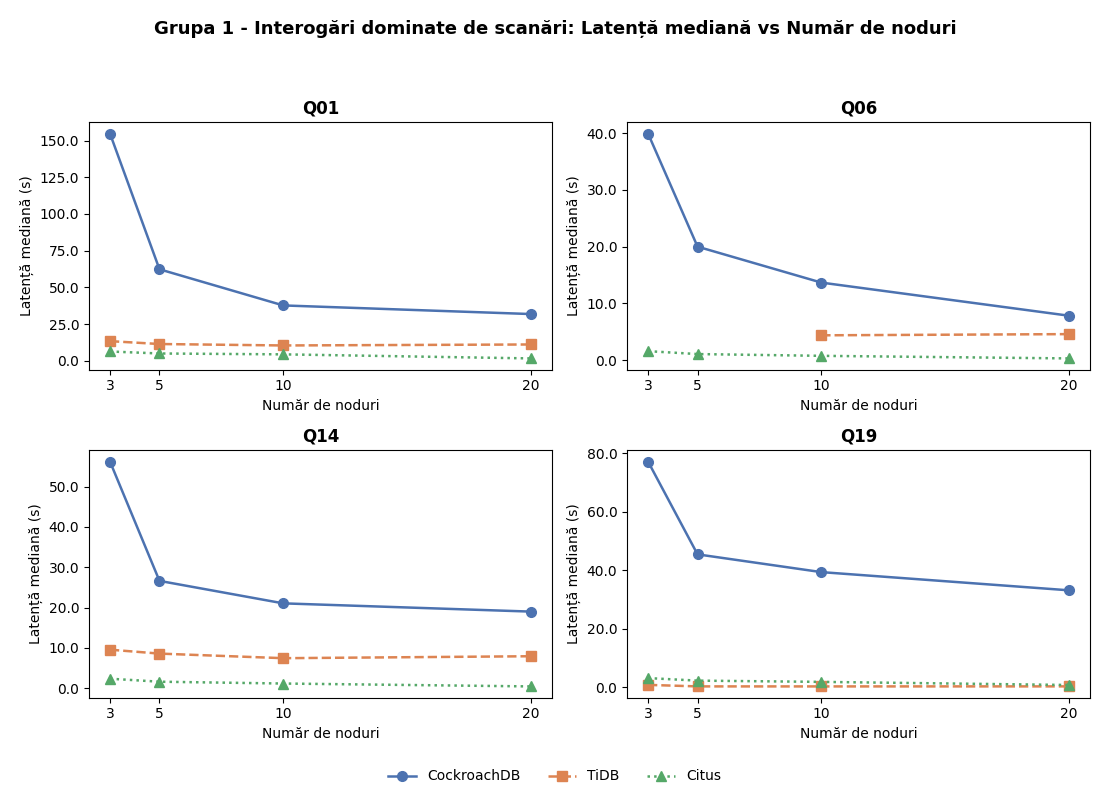
\includegraphics[width=\textwidth]{fig/g1_latency_vs_nodes.png}
    \caption{Grupa 1 - Interogări dominate de scanări: latența mediană în funcție de numărul de noduri pentru fiecare interogare.}
    \label{fig:g1_latency_vs_nodes}
\end{figure}

\begin{figure}[H]
    \centering
    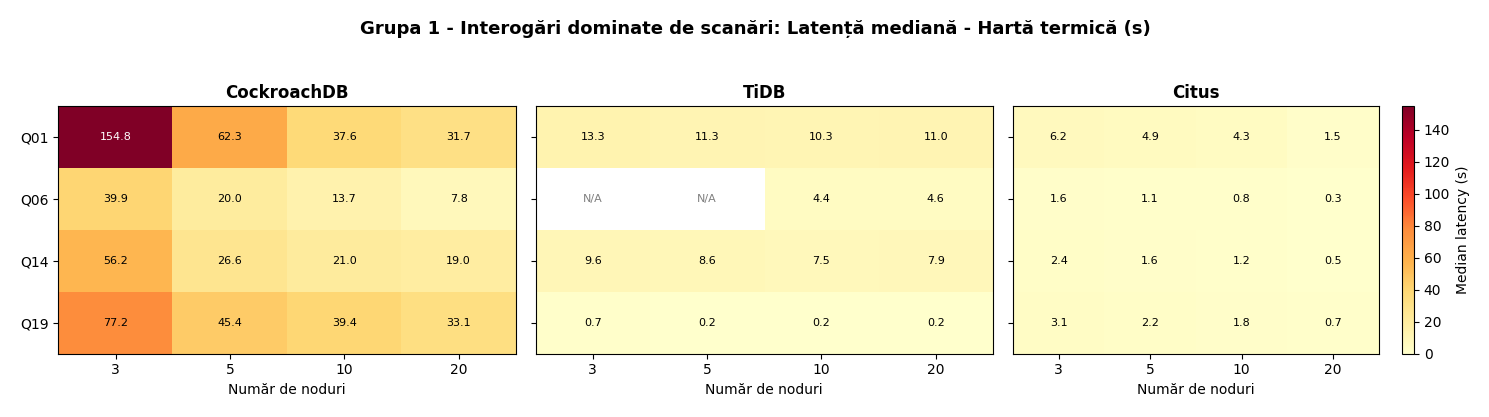
\includegraphics[width=\textwidth]{fig/g1_heatmap.png}
    \caption{Grupa 1 - Interogări dominate de scanări: harta termică a latenței mediane (secunde) pe matricea sistem $\times$ număr de noduri.}
    \label{fig:g1_heatmap}
\end{figure}

Figura \ref{fig:g1_latency_vs_nodes} și harta termică din figura \ref{fig:g1_heatmap} arată o ierarhie consistentă a latenței mediane. Citus este cel mai rapid sistem la fiecare combinație măsurată. TiDB se situează la mijloc, iar CockroachDB are cea mai mare latență cu o marjă semnificativă. Se poate observa o diferență majoră la configurația de 3 noduri, Q1 rulează în $6,2\approx$ secunde pe Citus și în $13,3\approx$ secunde pe TiDB, dar necesită $154,8\approx$ secunde pe CRDB, un factor de aproximativ 25$\times$ în defavoarea acestuia. Aceste tipare se observă și pe Q14 ($2,4$ vs $9,6$ vs $56,2\approx$ secunde) și pe Q19 ($0,7$ vs $3,1$ vs $77,2\approx$ secunde). Este de notat că la Q19 TiDB se aproprie de performanța Citus. La configurația cea mai puternică, cea de 20 de noduri distanța dintre CRDB și restul sistemelor se reduce dar nu se elimină, ierarhia rămâne aceeași pe toate interogările din acest grup.

\begin{figure}[H]
    \centering
    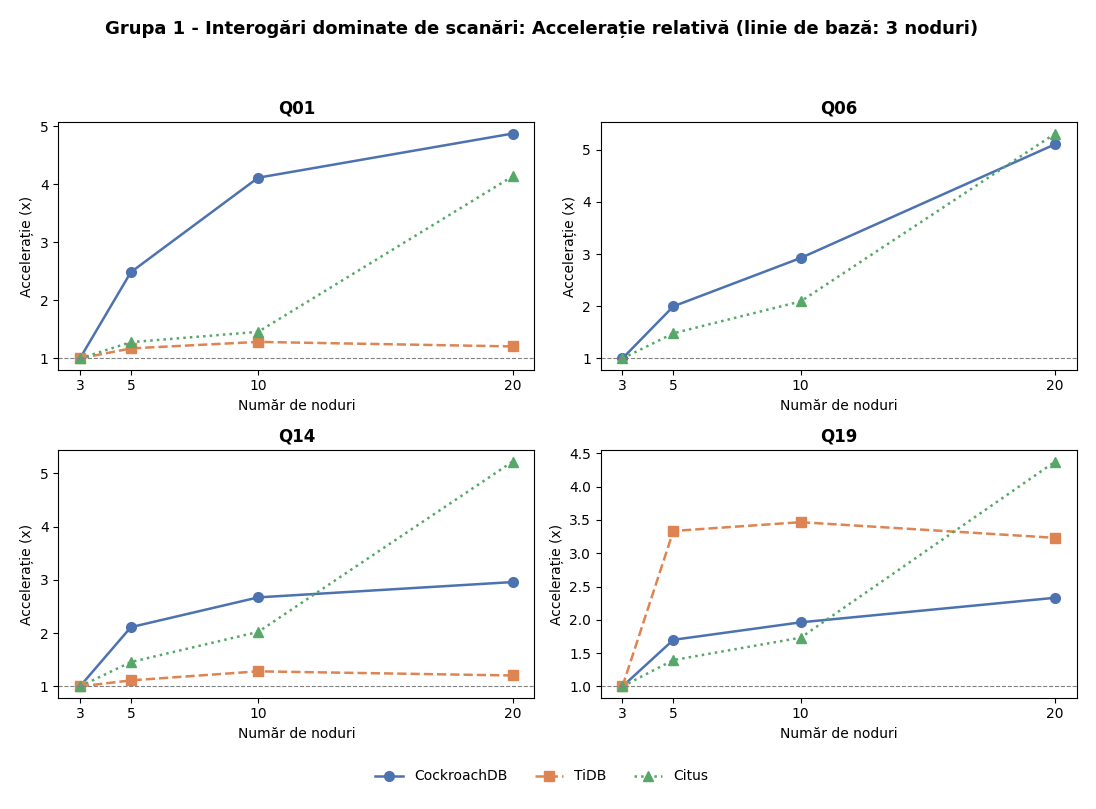
\includegraphics[width=\textwidth]{fig/g1_speedup.png}
    \caption{Grupa 1 - Interogări dominate de scanări: accelerația relativă la linia de bază cu 3 noduri.}
    \label{fig:g1_speedup}
\end{figure}

Analiza accelerației relative la configurația de 3 noduri, prezentată în figura \ref{fig:g1_speedup}, completează imaginea. CockroachDB prezintă cea mai pronunțată accelerație în această grupă, atingând chiar un factor de aproximativ $4,9\times$ pe Q1 și $5.1\times$ pe Q6. Citus prezintă un comportament similar. Această observație este interesantă, aproape contradictorie cu analiza latențelor dar este revenită din planurile de execuție. CockroachDB scalează bine pentru că pornește de la o bază lentă, cu mult spațiu disponibil pentru paralelizare. În contrast, TiDB prezintă o accelerație destul de slabă, singura excepție fiind reprezentată de Q19, unde TiDB atinge $3,4\times$ accelerație la 5 noduri, dar apoi se stabilizează, indicând o îmbunătățire provenită din nivelul de paralelizare.

\begin{figure}[H]
    \centering
    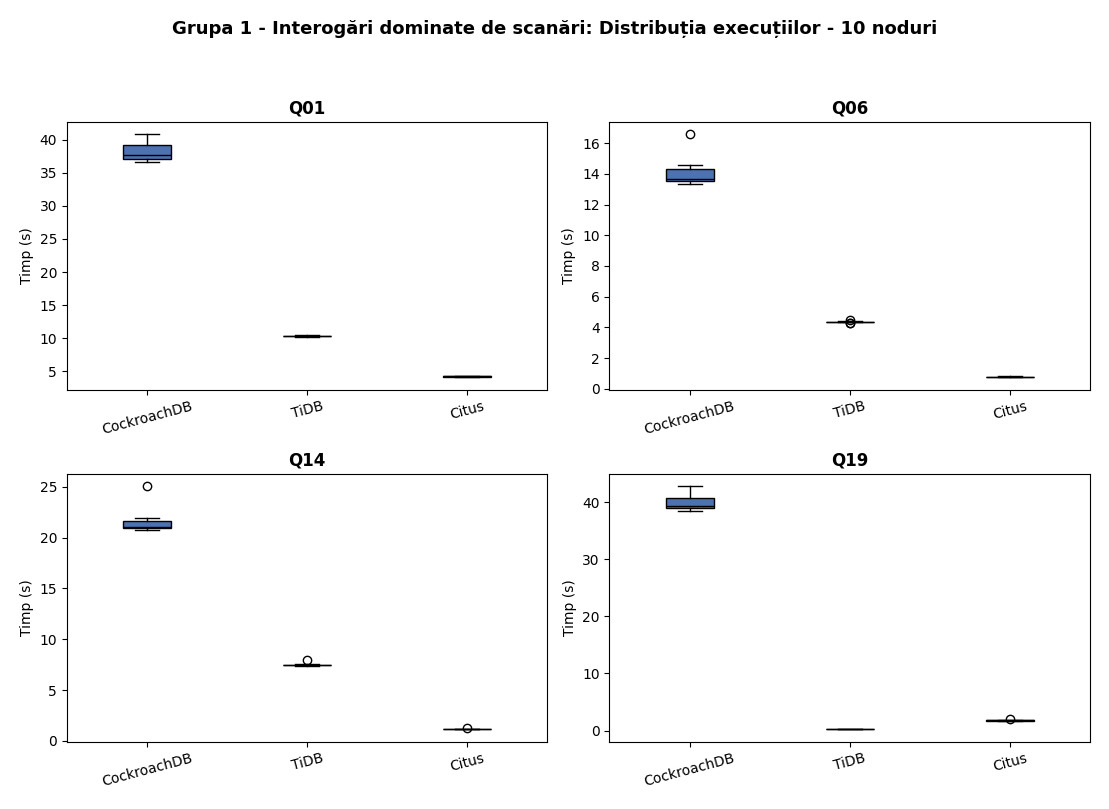
\includegraphics[width=\textwidth]{fig/g1_boxplots_10n.png}
    \caption{Grupa 1 - Interogări dominate de scanări: distribuția celor zece rulări temporizate la configurația cu 10 noduri.}
    \label{fig:g1_boxplots_10n}
\end{figure}

Distribuția rulărilor la 10 noduri, prezentată în figura~\ref{fig:g1_boxplots_10n}, indică o variabilitate scăzută pentru
toate cele trei sisteme pe această grupă. Diagramele de tip cutie sunt foarte strâmte pe TiDB și pe Citus, sugerând că aceste sisteme produc durate de execuție extrem de reproductibile pentru interogările dominate de scanări. CRDB prezintă cutii ușor mai late și cu valori aberante ocazional, dar variația rămâne sub 10 \% din mediana.

Există două abateri notabile de la tiparul general. Prima este absența datelor pentru Q6 pe TiDB la configurațiile cu 3 și 5 noduri, marcată „N/A” în figura~\ref{fig:g1_heatmap}. Această absență nu reflectă un comportament arhitectural al sistemului, ci un eșec de colectare a planului la acele puncte specifice de măsurare, datorat unei erori OOM. A doua abatere este Q19, unde TiDB devansează atât CockroachDB cât și Citus în absolut, cu latențe sub o secundă la toate configurațiile de peste 3 noduri.

\section{Grupa 2 - Interogări dominate de îmbinări}

Cea de a doua grupă este formată din interogările Q3, Q5, Q7, Q8, Q9 și Q10, care combină tabelele \texttt{lineitem} și \texttt{orders} cu mai multe tabele de dimensiuni diferite prin join-uri multiple. Specific acestei categorii este costul dominant provenit din execuția unui graf de îmbinări, care implică între 3 și 6 tabele simultan. Această grupă prezintă comportamentul fiecărui sistem la nivel arhitectural prin strategia de partiționare și capacitatea planificatorului de a alege un algoritm de join optim pentru a exploata co-localizarea datelor.

\begin{figure}[H]
    \centering
    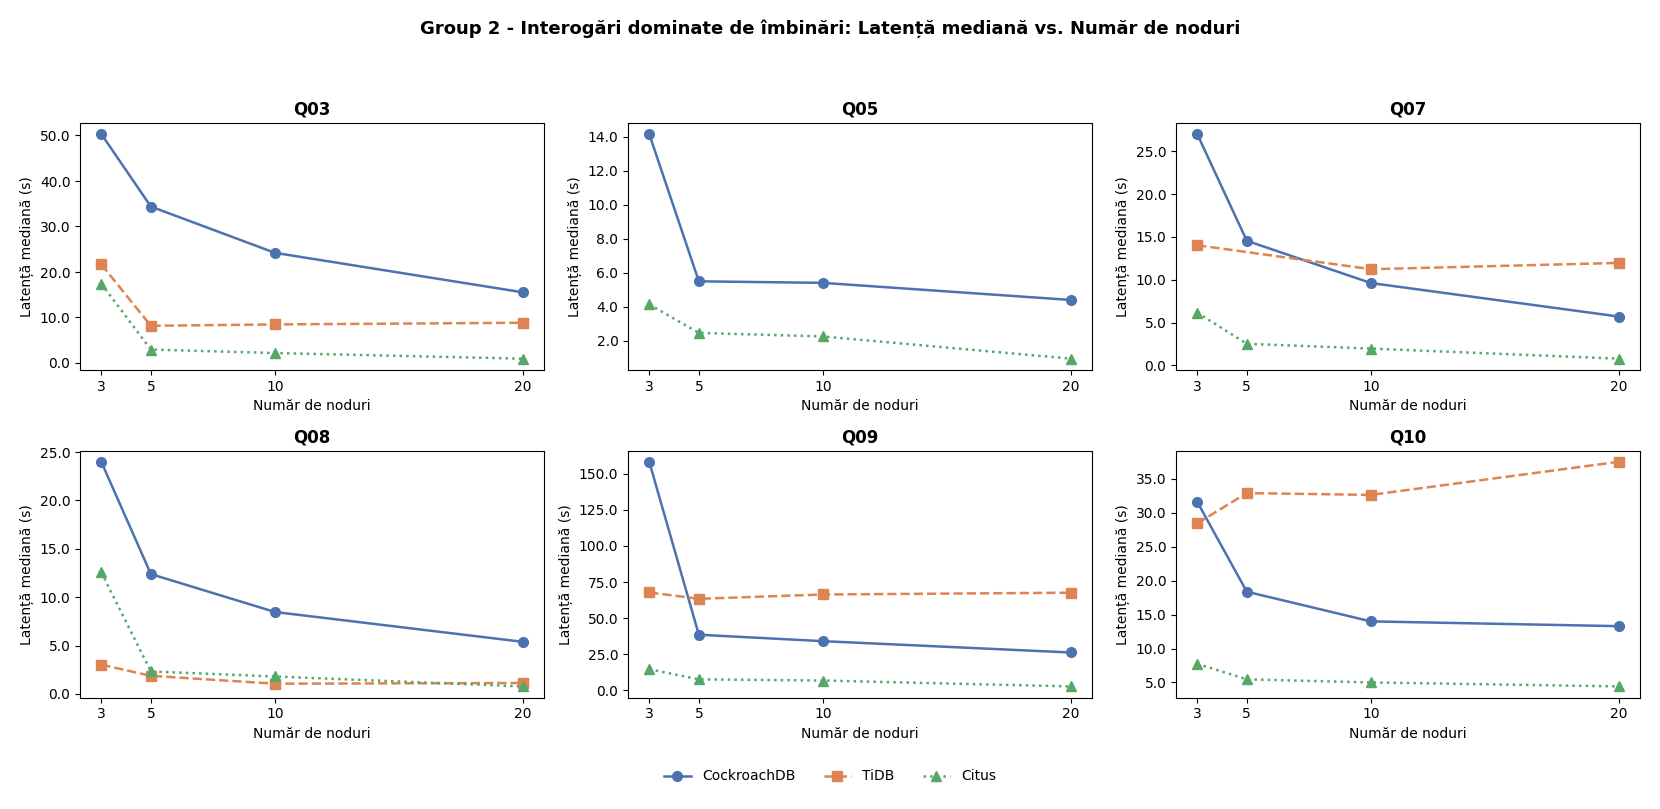
\includegraphics[width=\textwidth]{fig/g2_latency_vs_nodes.png}
    \caption{Grupa 2 - Interogări dominate de îmbinări: latența mediană în funcție de numărul de noduri.}
    \label{fig:g2_latency_vs_nodes}
\end{figure}

\begin{figure}[H]
    \centering
    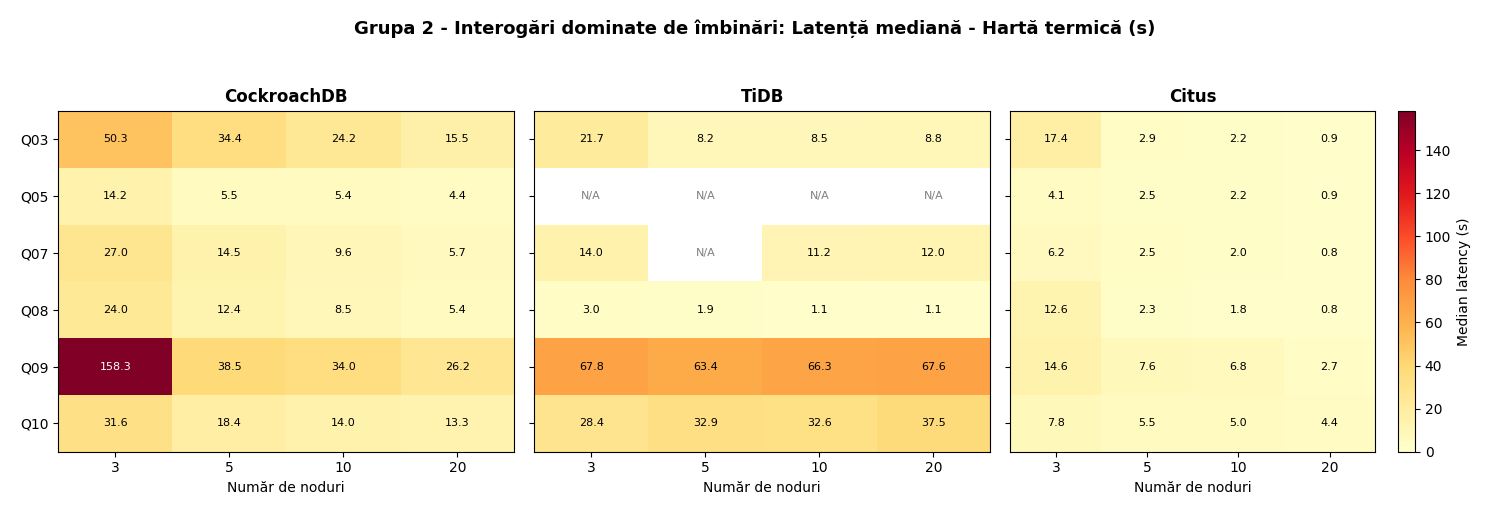
\includegraphics[width=\textwidth]{fig/g2_heatmap.png}
    \caption{Grupa 2 - Interogări dominate de îmbinări: harta termică a latenței mediane (secunde).}
    \label{fig:g2_heatmap}
\end{figure}

Figura \ref{fig:g2_latency_vs_nodes} și harta termică din figura \ref{fig:g2_heatmap} arată o ierarhie de performanță care este total diferită de cea din grupa precedentă. Citus rămâne în continuare sistemul cu cea mai mică latență, cu un avantaj mai ales pe Q3 (17,4 vs 21,7 vs $50,3\approx$ secounde) respectiv 0,9 vs 8,8 vs 15,5$\approx$ secunde în configurația de 20 de noduri. În schimb, raportul dintre TiDB și CockroachDB se inversează față de prima grupa, pentru cele mai multe interogări din această grupă CRDB are latențe mai mici decât TiDB la configurațiile cu 5, 10 și 20 de noduri. Observăm pe Q9 cum CockroachDB scade de la $158,3\approx$ secunde în configurația de 3 noduri la $26,2\approx$ secunde în configurația de 20 de noduri, în timp ce TiDB stagnează în jurul valorii de $66\approx$ secunde în toate configurațiile. Tipare similare observă și la Q7 și Q10. Această observație reflectă diferența fundamentală dintre sarciniile dominate de scanare (unde pushdown-ul de agregare către stratul de stocare - TiKV este factorul decisiv) și sarcinile dominate de join-uri (unde algoritmul de îmbinare la stratul de execuție este factorul decisiv).

\begin{figure}[H]
    \centering
    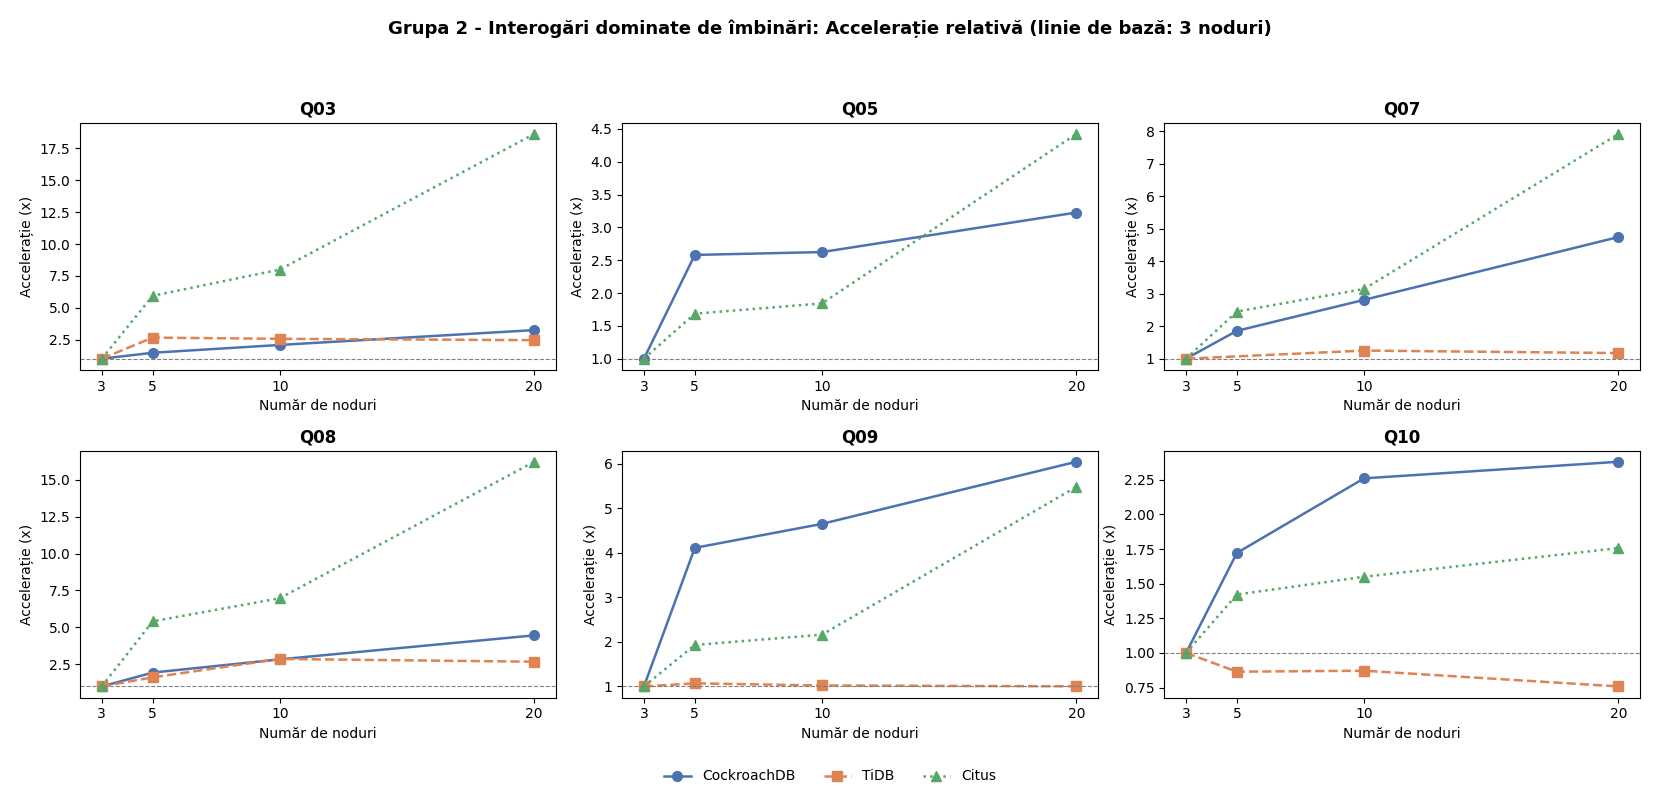
\includegraphics[width=\textwidth]{fig/g2_speedup.png}
    \caption{Grupa 2 - Interogări dominate de îmbinări: accelerația relativă la linia de bază cu 3 noduri.}
    \label{fig:g2_speedup}
\end{figure}

Analiza accelerației din figura~\ref{fig:g2_speedup} amplifică această diferență. Citus prezintă factorii de accelerație cei mai mari din întreg studiul pe interogările Q3 (aproximativ 19$\times$ la 20 de noduri) și Q8 (aproximativ 16$\times$), iar CockroachDB înregistrează accelerații robuste pe majoritatea interogărilor din grupă, atingând 6$\times$ pe Q9 și aproximativ 5$\times$ pe Q7. Se poate observa comportamentul TiDB pe această grupă, unde pe Q8, factorul de accelerație rămâne practic egal cu 1 pe toate configurațiile, iar pe Q10 apare o regresie a performanței pe măsură ce numărul de noduri crește. Această observație este o consecință directă a algoritmului de join ales de sistemul TiDB.

\begin{figure}[H]
    \centering
    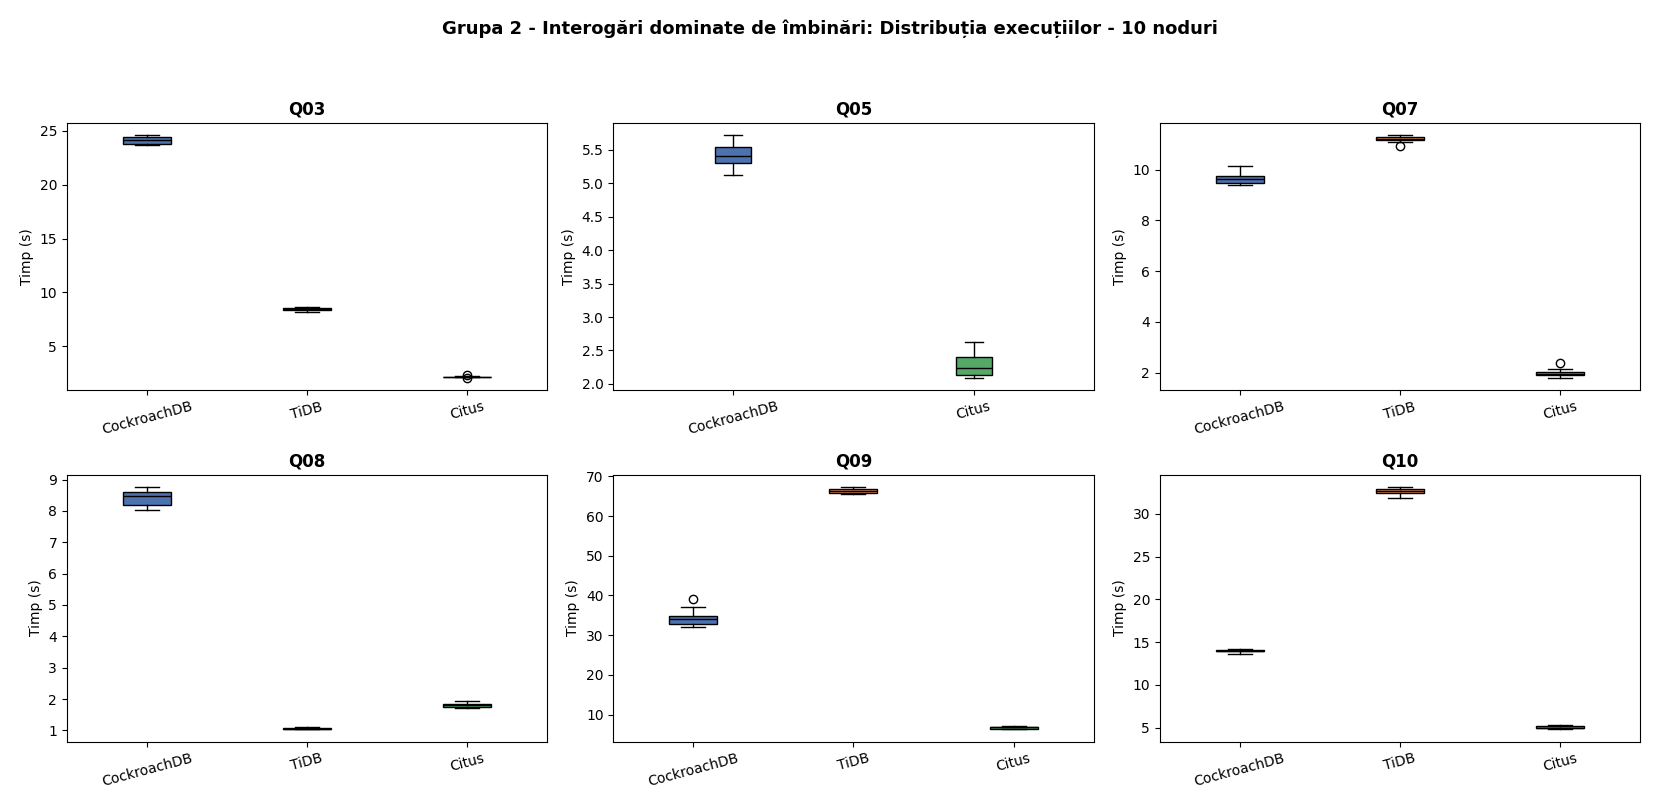
\includegraphics[width=\textwidth]{fig/g2_boxplots_10n.png}
    \caption{Grupa 2 - Interogări dominate de îmbinări: distribuția celor zece rulări temporizate la configurația cu 10 noduri.}
    \label{fig:g2_boxplots_10n}
\end{figure}

Distribuția rulărilor la 10 noduri, prezentată în figura~\ref{fig:g2_boxplots_10n}, confirmă că diferențele de latență observate sunt structurale și nu efecte ale variabilității. Cutiile sunt strâmte pentru toate cele trei sisteme pe majoritatea interogărilor, cu amplitudini relative sub 5\%.

\section{Grupa 3 - Interogări conduse de subinterogări}

A treia grupă reunește interogările Q2, Q11, Q17 și Q22, fiecare dintre aceste interogări fiind caracterizare printr-o subinterogare corelată sau printr-o agregare cu un subansamblu derivat din tabele exterioare (de bază). Q2 se folosește de o subinterogare corelată pe \texttt{partsupp} pentru a căuta furnizorul cu costul minim pentru fiecare combinație între piesă și regiune. Q11 folosește o subinterogare scalară tot pe \texttt{partsupp} pentru a calcula piesele a căror valoare totală în stoc depășește un anumit prag. Q17 calculează venitul mediu pe piese cu cantități sub un prag derivat din media aceleiași tabele \texttt{lineitem}. Q22 segmentează clienții fără comenzi după zona telefonică, după filtrarea pe baza unei medii globale a soldului. În toate aceste cazuri, planul logic include cel puțin o subinterogare al cărei rezultat trebuie decorelat sau materializat înainte de a putea fi folosit în îmbinarea principală, iar performanța depinde critic de strategia aleasă de optimizator pentru această materializare.

\begin{figure}[H]
    \centering
    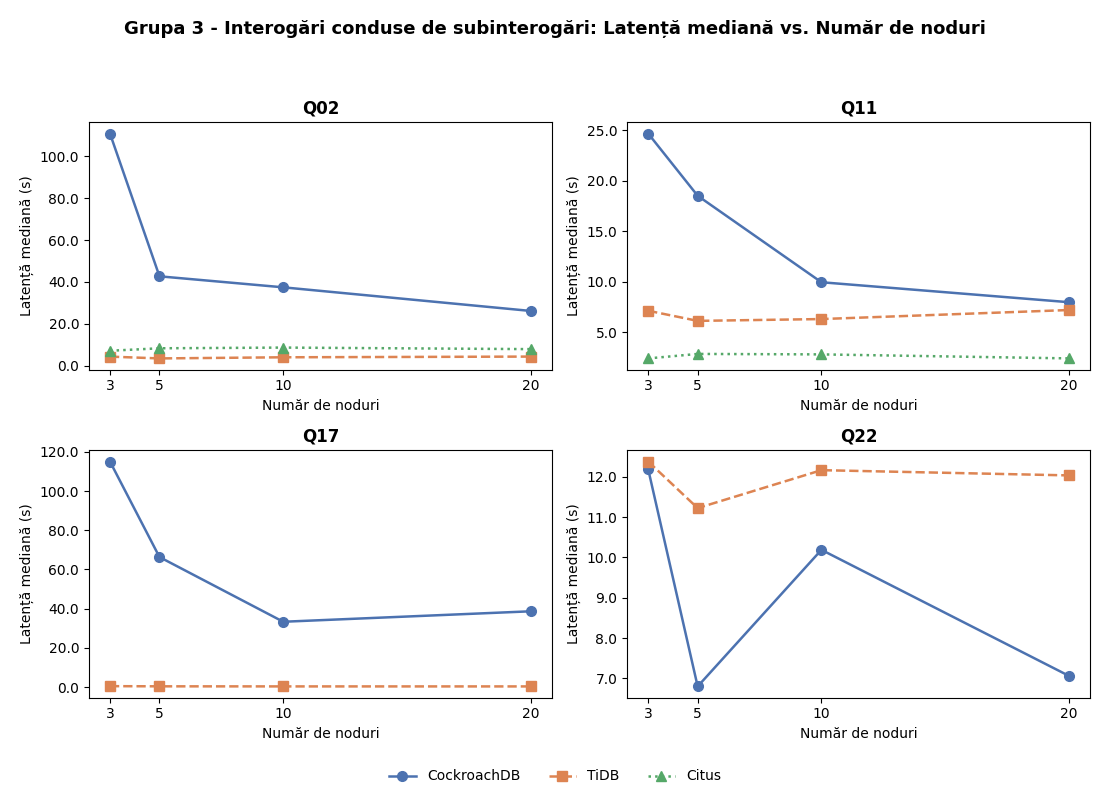
\includegraphics[width=\textwidth]{fig/g3_latency_vs_nodes.png}
    \caption{Grupa 3 - Interogări conduse de subinterogări: latența mediană în funcție de numărul de noduri.}
    \label{fig:g3_latency_vs_nodes}
\end{figure}

\begin{figure}[H]
    \centering
    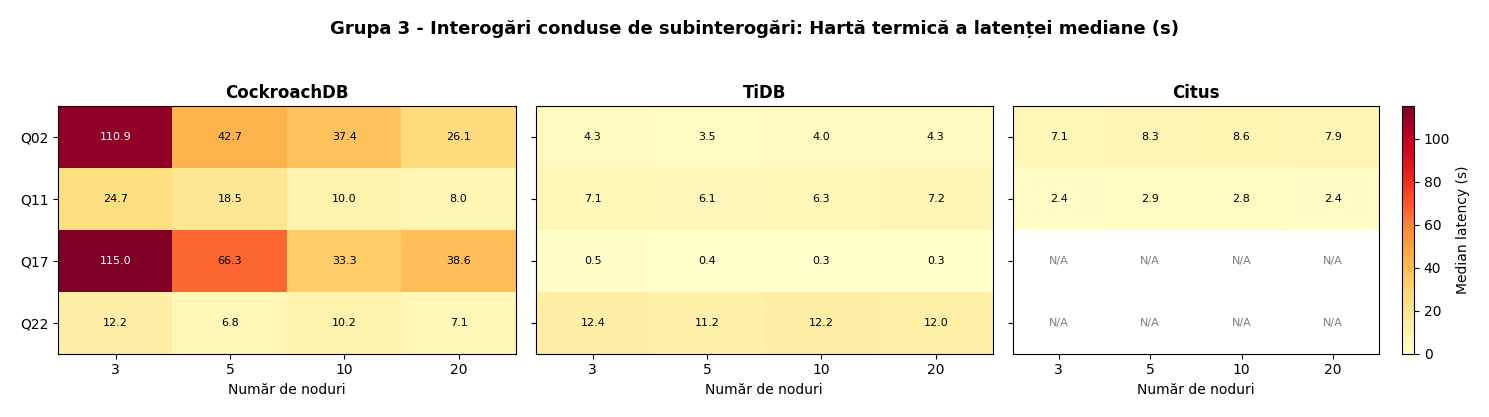
\includegraphics[width=\textwidth]{fig/g3_heatmap.png}
    \caption{Grupa 3 - Interogări conduse de subinterogări: harta termică a latenței mediane (secunde).}
    \label{fig:g3_heatmap}
\end{figure}

Figura \ref{fig:g3_latency_vs_nodes} și harta termică din figura \ref{fig:g3_heatmap} arată o performanță împărțită, fragmentată, fără un câștigător consistent: fiecare sistem domină pe câte o interogare diferită din grupă. TiDB este sistemul cu cea mai mică latență absolută pe Q2 ($3,5-4,3\approx$ secunde la toate configurațiile) și pe Q17 (unde latența scade sub o secundă la toate configurațiile, $0,3-0,5\approx$ secunde). Citus este cel mai rapid pe Q11 ($2,4-2,9\approx$ secunde) acolo unde poate executa interogarea, dar \textbf{nu produce rezultate pe Q17 și Q22}. CockroachDB pierde clar pe Q2 și Q17 la 3 noduri (110,9
respectiv 115,0$\approx$secunde) dar recuperează semnificativ prin paralelism. Fragmentarea pe această grupă nu este arbitrară, ea reflectă diferențele profunde dintre strategiile fiecărui planificator de a procesa subinterogări corelate.

\begin{figure}[H]
    \centering
    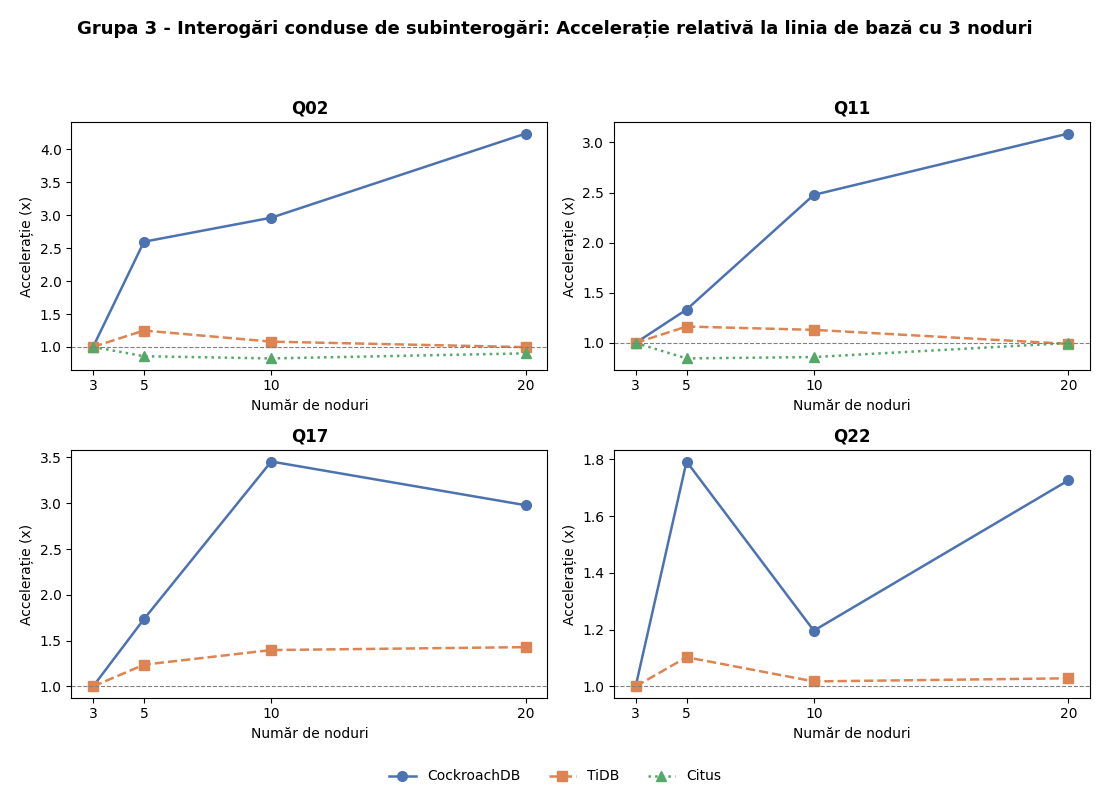
\includegraphics[width=\textwidth]{fig/g3_speedup.png}
    \caption{Grupa 3 - Interogări conduse de subinterogări: accelerația relativă la linia de bază cu 3 noduri.}
    \label{fig:g3_speedup}
\end{figure}

Analiza accelerației din figura~\ref{fig:g3_speedup} este profund asimetrică între sisteme. CockroachDB prezintă cele mai pronunțate accelerații din grupă, atingând aproximativ 4,2$\times$ pe Q2 și 3,4$\times$ pe Q17 la 10 noduri (urmate de o regresie ușoară la 20 de noduri pe Q17. TiDB rămâne practic plat la toate cele patru interogări, cu accelerații sub 1,4$\times$ chiar și la 20 de noduri. Citus, în mod cel mai surprinzător, prezintă accelerații nule sau ușor sub-unitare pe Q2 și Q11 (factorul $0,9-1,0\times$ la toate configurațiile), comportament care diferă radical de tiparul scalabil observat pe primele două grupe.

\begin{figure}[H]
    \centering
    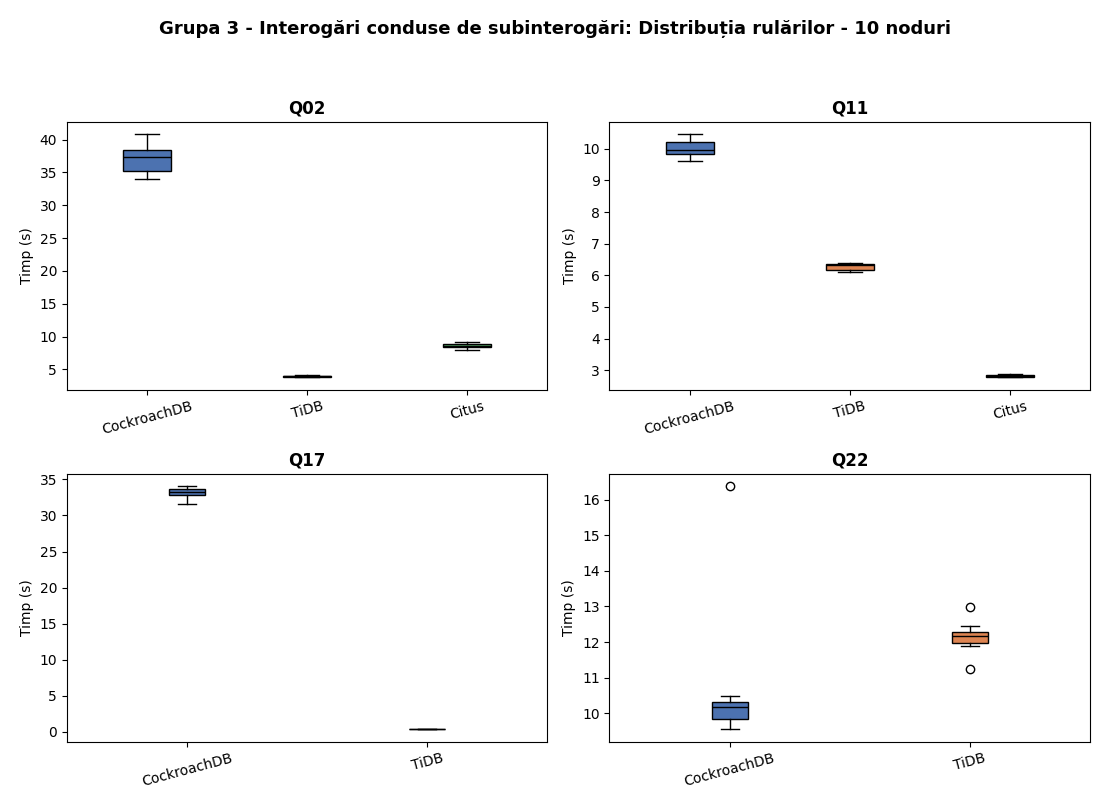
\includegraphics[width=\textwidth]{fig/g3_boxplots_10n.png}
    \caption{Grupa 3 - Interogări conduse de subinterogări: distribuția celor zece rulări temporizate la configurația cu 10 noduri.}
    \label{fig:g3_boxplots_10n}
\end{figure}

Distribuția rulărilor la 10 noduri, prezentată în figura~\ref{fig:g3_boxplots_10n}, este în general strâmtă, cu o singură excepție notabilă: CockroachDB pe Q22 prezintă o valoare aberantă clară la aproximativ 16~secunde, în timp ce restul rulărilor sunt concentrate în jurul valorii de 10~secunde. Această valoare aberantă unică explică și tiparul non-monoton observat în figura~\ref{fig:g3_latency_vs_nodes} pentru Q22 pe CockroachDB (12,2~$\rightarrow$~6,8~$\rightarrow$~10,2~$\rightarrow$~7,1~secunde pe măsura creșterii numărului de noduri).

\section{Grupa 4 - Interogări în mai multe etape}

A patra grupă este cea mai complexă și diferită din studiu, formată din Q4, Q12, Q13, Q15, Q16, Q18, Q20 și Q21, cuprinzând opt interogări care combină tehnici relaționale diverse: agregări nestate, join-uri auto-referențiale, expresii de tabel comune (CTE), îmbinări laterale, precum și anti-join-uri. Q4 și Q12 efectuează agregări cu condiții de existență pe \texttt{lineitem}, Q13 calculează distribuția numărului de comenzi pe client printr-o îmbinare exterioară urmată de agregare în două etape, Q15 folosește o expresie CTE pentru a precalcula veniturile pe furnizor înainte de a identifica furnizorul cu venit maxim, Q16 calculează numărul de furnizori distincți pe combinație de proprietăți ale părților, Q18 identifică clienții cu cele mai mari comenzi printr-o îmbinare laterală, Q20 selectează furnizorii cu stocuri excedentare pentru o națiune dată, iar Q21 detectează furnizorii responsabili de livrări întârziate printr-o auto-îmbinare a tabelei \texttt{lineitem} cu construcții \texttt{EXISTS} și \texttt{NOT EXISTS}. Diversitatea grupei face ca observațiile generale să fie mai puțin uniforme de la o interogare la alta.

\begin{figure}[H]
    \centering
    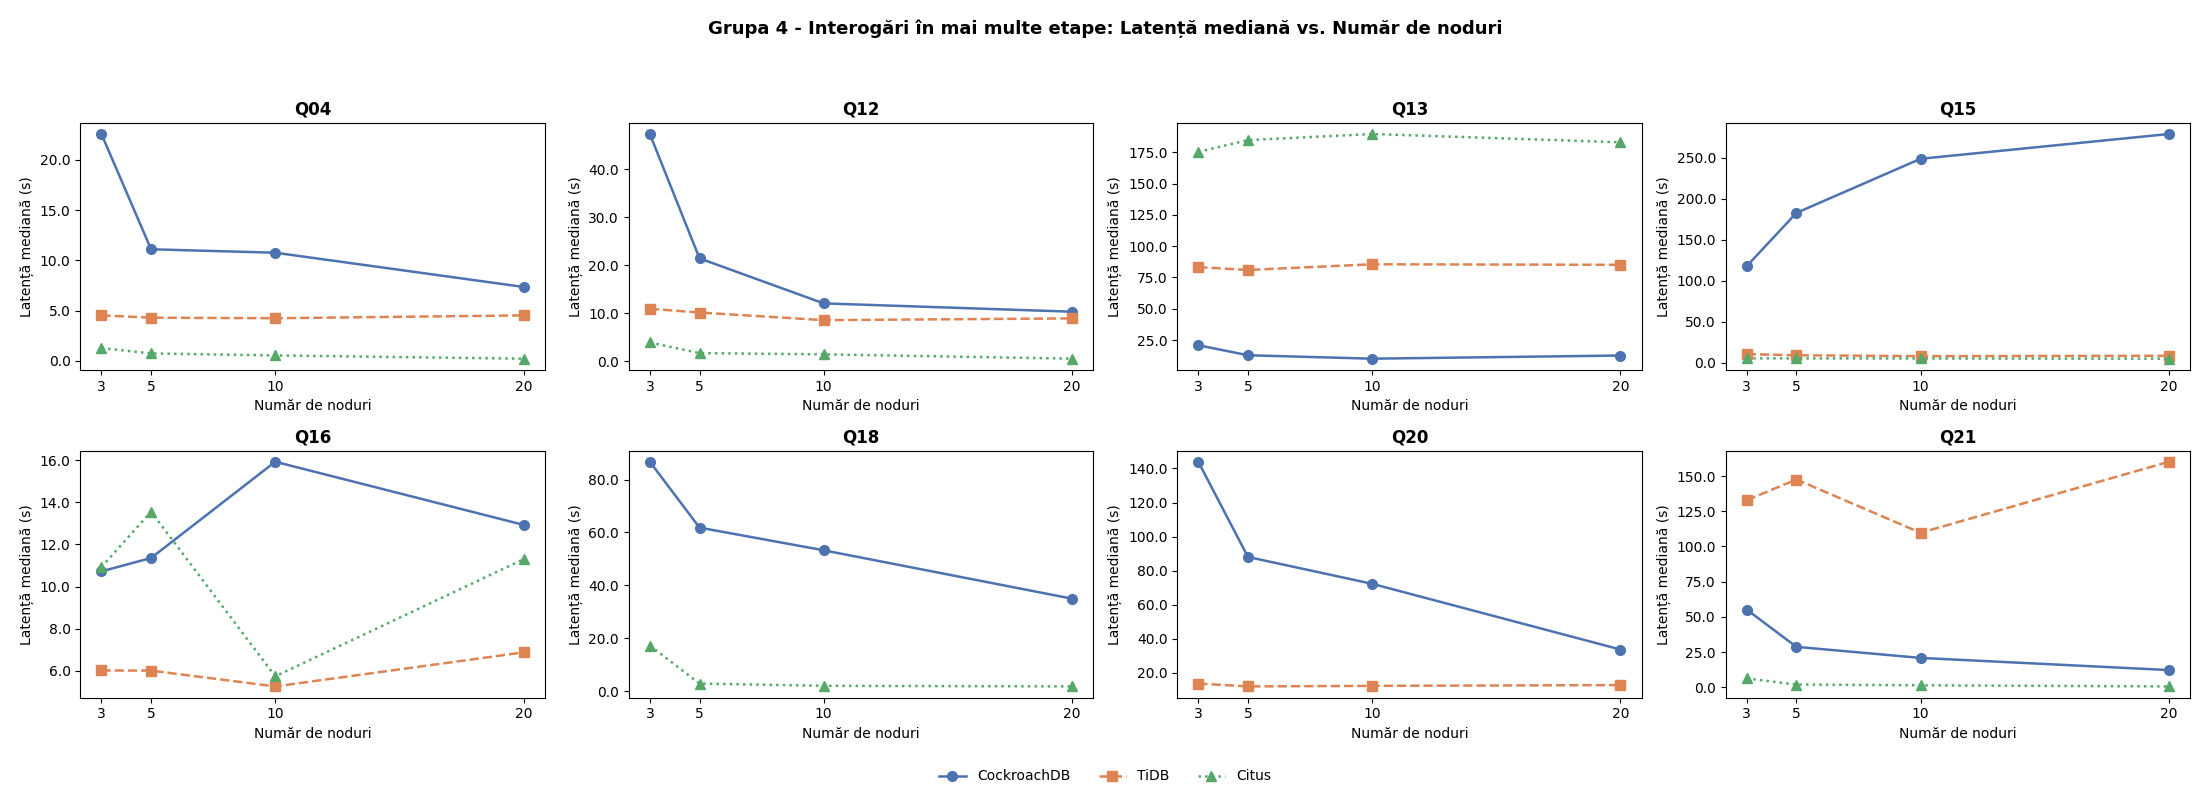
\includegraphics[width=\textwidth]{fig/g4_latency_vs_nodes.png}
    \caption{Grupa 4 - Interogări în mai multe etape: latența mediană în funcție de numărul de noduri.}
    \label{fig:g4_latency_vs_nodes}
\end{figure}

\begin{figure}[H]
    \centering
    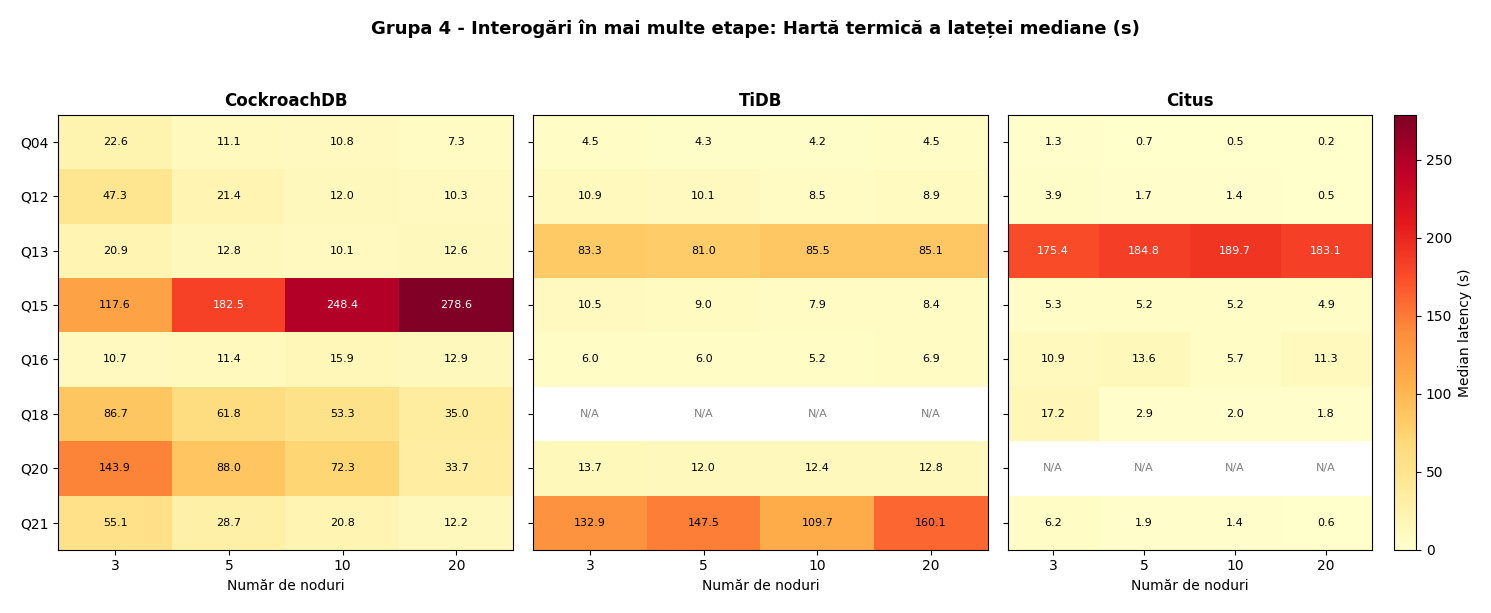
\includegraphics[width=\textwidth]{fig/g4_heatmap.png}
    \caption{Grupa 4 - Interogări în mai multe etape: harta termică a latenței mediane (secunde).}
    \label{fig:g4_heatmap}
\end{figure}

Figura \ref{fig:g4_latency_vs_nodes} și harta termică din figura \ref{fig:g4_heatmap} arată o dispersie a performanței mult mai mare decât pe grupele precedente, fără un câștigător dominant. Citus oferă dinnou cea mai mică latență absolută pe Q4, Q12, Q18 și Q21 (Q21 fiind cazul cel mai spectaculos cu 0,6 secunde la 20 de noduri), dar înregistrează un eșec total pe Q13 unde latența rămâne staționară în jurul valorii de $180 \approx$ secunde indiferent de numărul de noduri. TiDB oferă rezultate competitive pe Q4, Q12 și Q16 dar prezintă două anti-tipare severe pe Q13 ($85\approx$ de secunde la toate configurațiile) și pe Q21 ($130--160 \approx$ secunde, valoare neobișnuit de mare). CockroachDB prezintă cea mai gravă anti-scalare din întreg benchmarkul pe Q15, cu latența crescând de la $117,6$ secunde la 3 noduri la $278,6$ secunde la 20 de noduri. În rest, CockroachDB se comportă rezonabil pe Q4, Q12, Q20 și Q21, iar rezultatul pe Q13 este în mod surprinzător mult mai bun decât Citus și TiDB.

\begin{figure}[H]
    \centering
    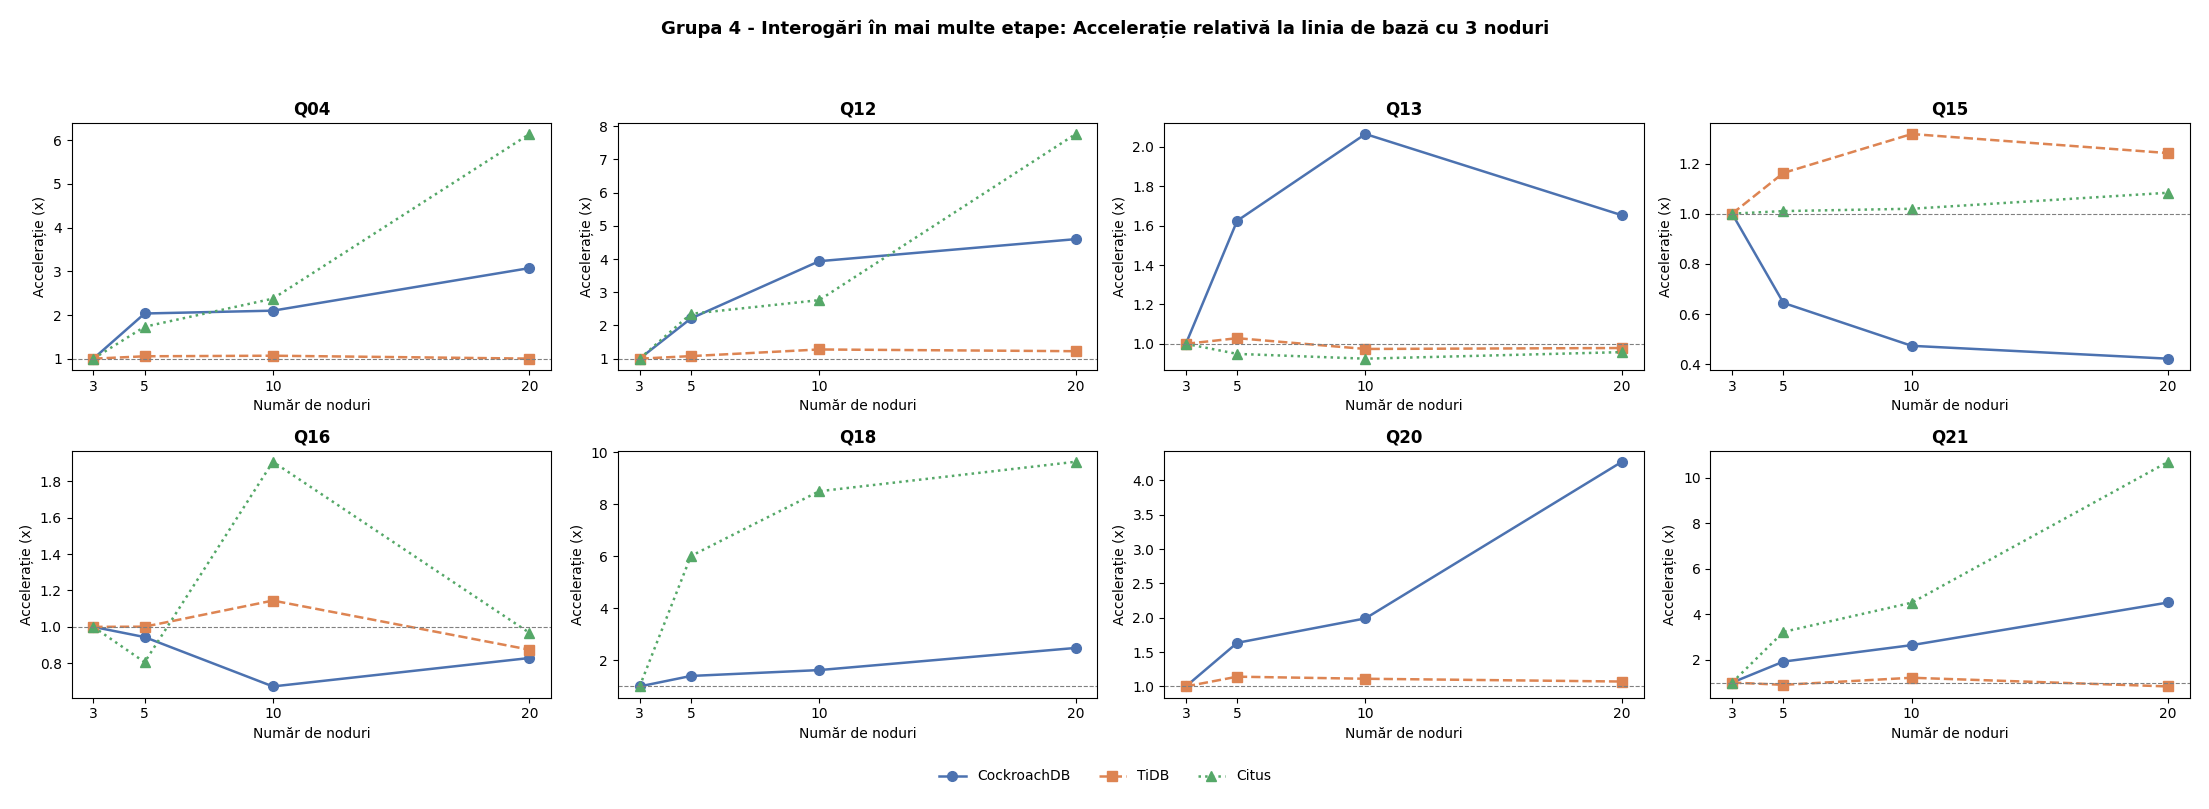
\includegraphics[width=\textwidth]{fig/g4_speedup.png}
    \caption{Grupa 4 - Interogări în mai multe etape: accelerația relativă la linia de bază cu 3 noduri.}
    \label{fig:g4_speedup}
\end{figure}

Analiza accelerației din figura~\ref{fig:g4_speedup} amplifică contrastele observate. Citus prezintă cele mai puternice accelerații din grupă pe Q4, Q12, Q18 și Q21, atingând factori între 6$\times$ și 10$\times$ la 20 de noduri. CockroachDB scalează robust pe Q20 (4,3$\times$), Q21 (4,5$\times$) și Q12 (4,6$\times$), dar prezintă un caz unic de accelerație fundamental sub-unitară pe Q15, cu factor de aproximativ 0.42$\times$ la 20 de noduri, adică sistemul devine cu 58\% mai lent prin adăugarea de noduri. TiDB rămâne în mare parte plat pe această grupă, cu accelerații sub 1,3$\times$ pe șapte din cele opt interogări, cu excepția Q4 unde nici TiDB nu beneficiază semnificativ.

\begin{figure}[H]
    \centering
    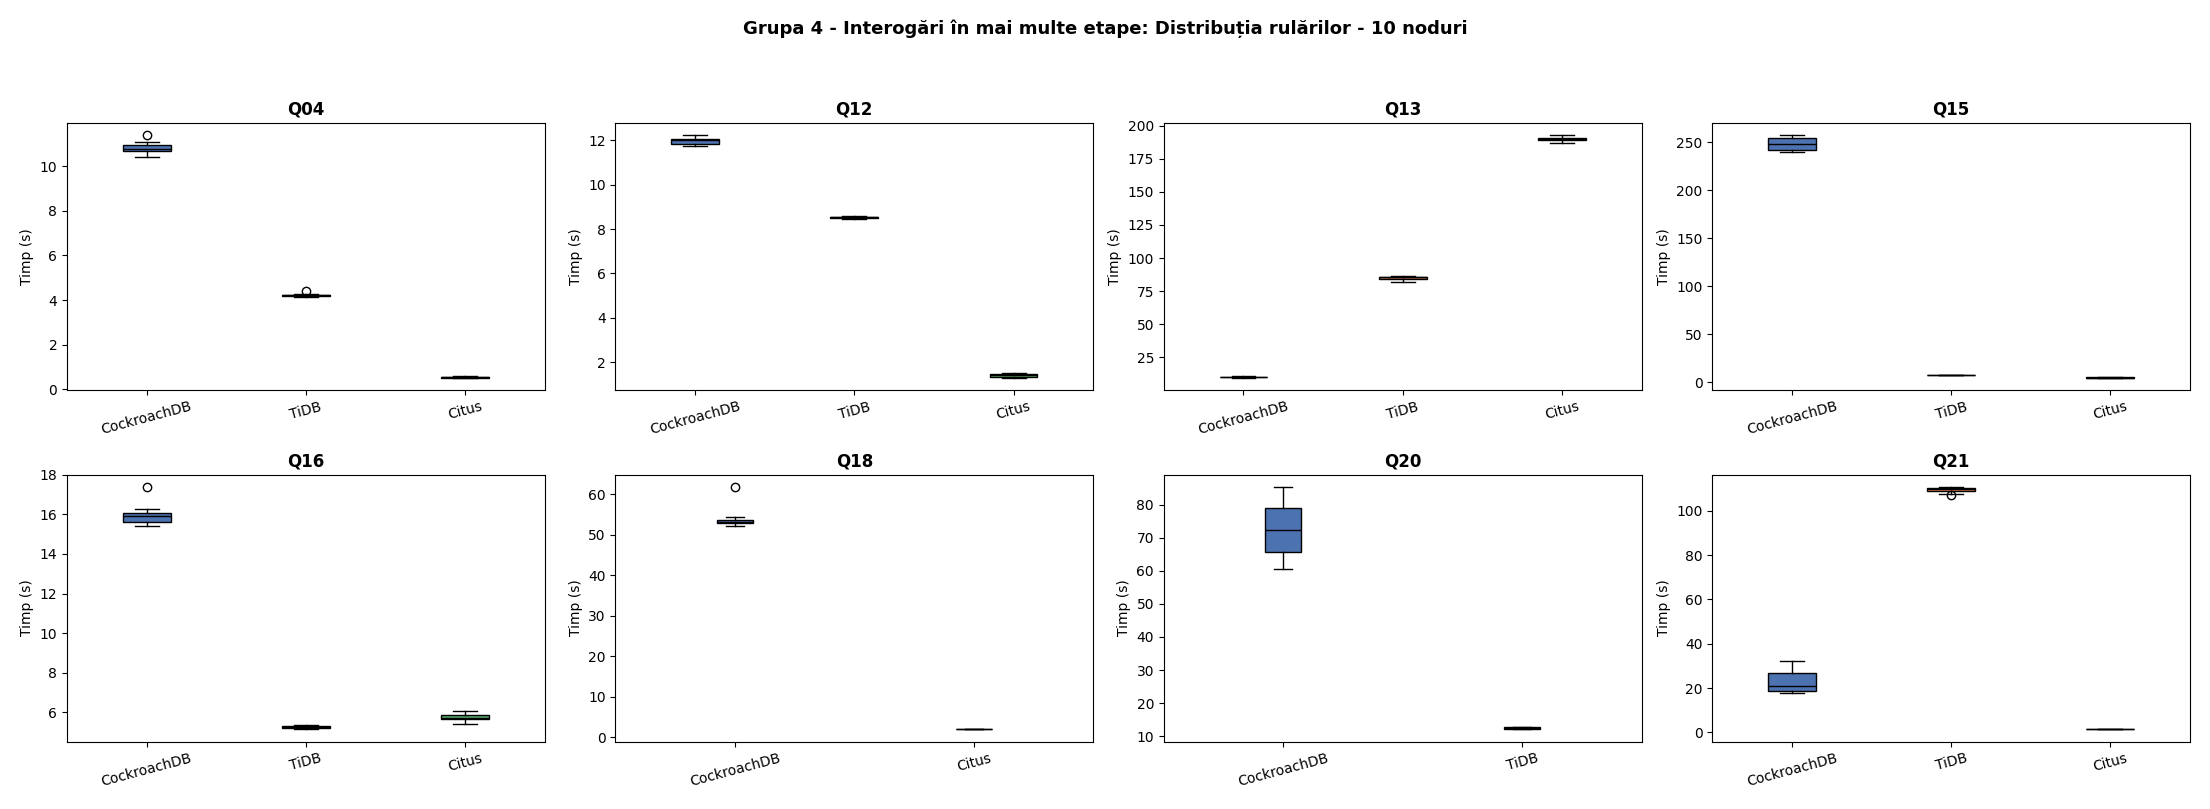
\includegraphics[width=\textwidth]{fig/g4_boxplots_10n.png}
    \caption{Grupa 4 - Interogări în mai multe etape: distribuția celor zece rulări temporizate la configurația cu 10 noduri.}
    \label{fig:g4_boxplots_10n}
\end{figure}

Distribuția rulărilor la 10 noduri, prezentată în figura \ref{fig:g4_boxplots_10n}, indică două cazuri de variabilitate crescută care merită atenție. Q16 prezintă pentru Citus o cutie cu amplitudine mai mare decât pe celelalte sisteme, sugerând că planul de execuție al acestei interogări produce rezultate inconsistente între rulări. Această observație este confirmată și de figura latenței (figura \ref{fig:g4_latency_vs_nodes}), care arată un tipar nelinear clar pentru Citus pe Q16 (10,9~$\rightarrow$,13,6~$\rightarrow$~5,7~$\rightarrow$~11,3~$\approx$ secunde). Q20 pe CockroachDB prezintă cea mai largă cutie din întreg studiul, cu interval de aproximativ 20 secunde și extreme de aproximativ 60 și 80 secunde.

\section{Sinteză intergrupală}

\begin{figure}[H]
    \centering
    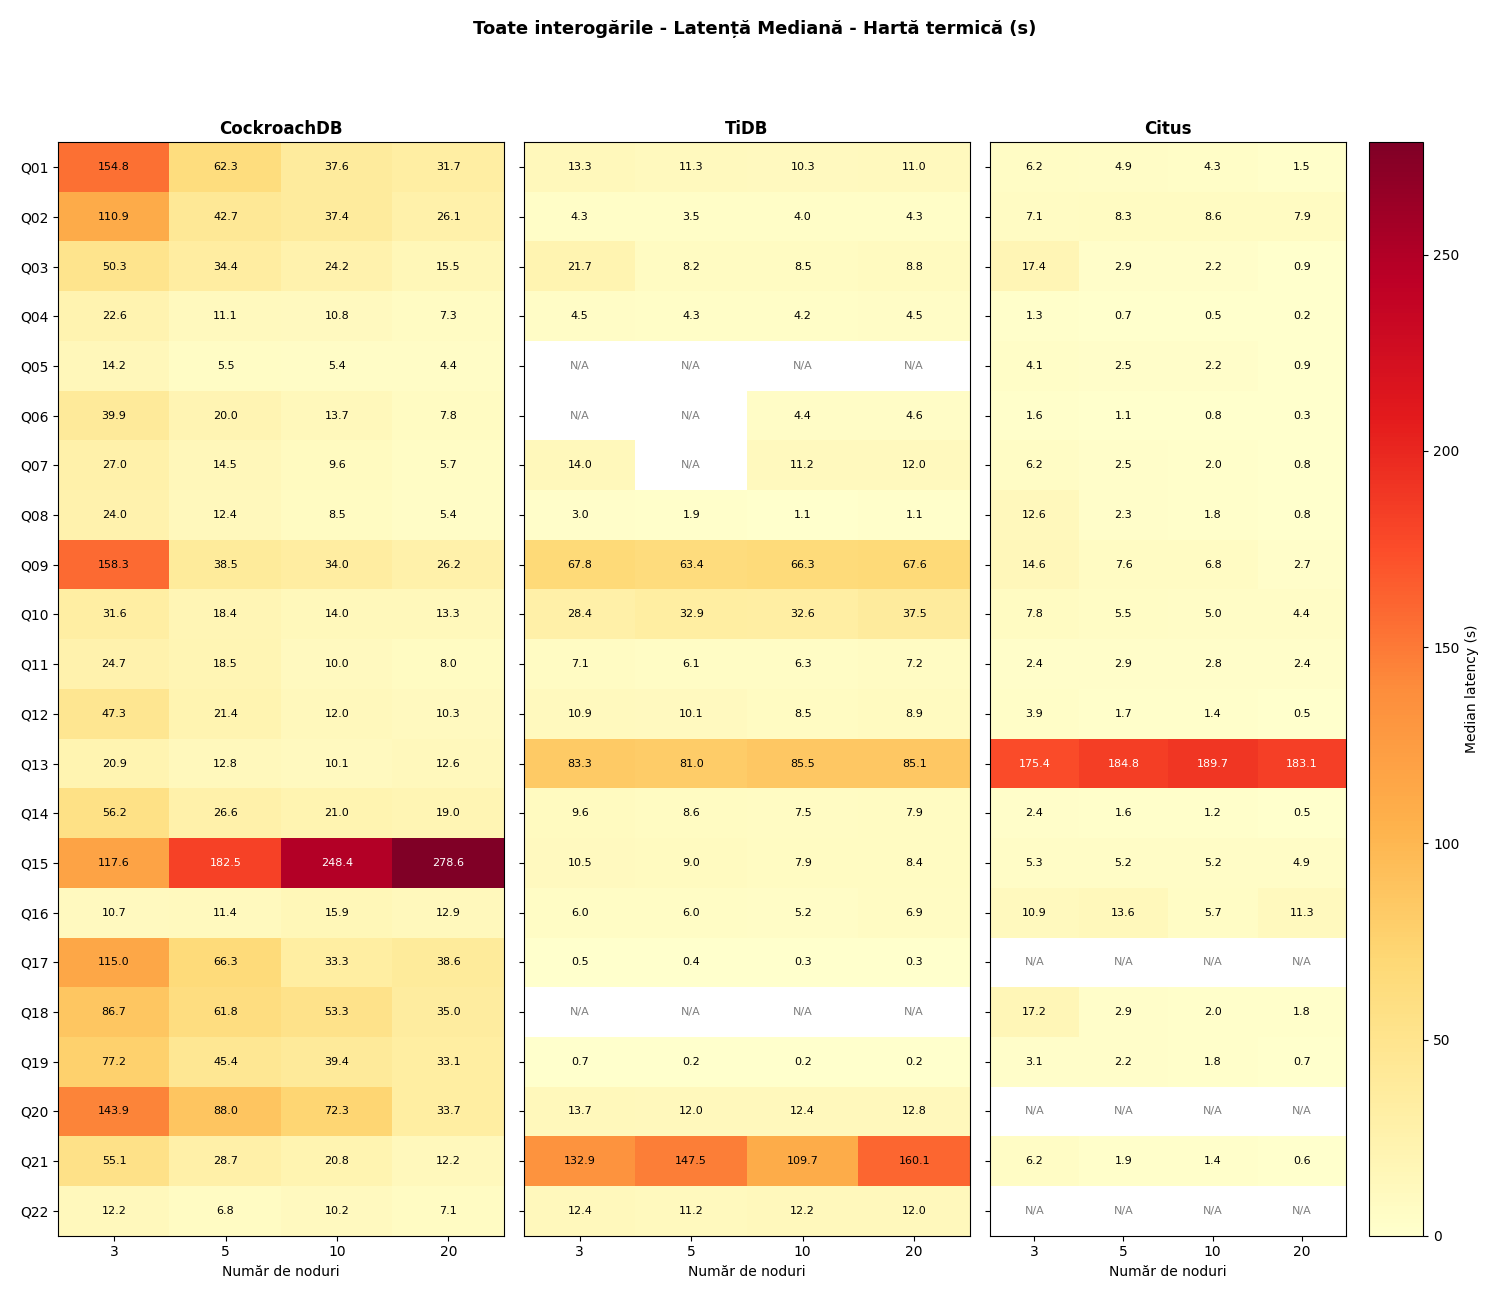
\includegraphics[width=\textwidth]{fig/global_heatmap.png}
    \caption{Harta termică globală a latenței mediane (secunde) pentru toate cele 22 de interogări TPC-H pe toate cele patru configurații de cluster.}
    \label{fig:global_heatmap}
\end{figure}

Harta termică globală din figura~\ref{fig:global_heatmap} oferă imaginea de ansamblu cea mai compactă a rezultatelor. Prima observație este acoperirea diferită a celor trei sisteme: CockroachDB execută toate
cele 22 de interogări la toate cele patru configurații, în timp ce TiDB nu produce rezultate pentru Q5 și Q18 la nicio configurație și prezintă lipsuri tranzitorii pe Q6 (configurațiile cu 3 și 5 noduri) și pe Q7 (configurația cu 5 noduri), iar Citus nu poate executa Q17, Q20 și Q22 din motive arhitecturale documentate în secțiunile precedente. Această diferență de acoperire constituie ea însăși un rezultat: pentru medii care prioritizează compatibilitatea SQL strictă cu specificația TPC-H peste performanța de vârf, CockroachDB este singurul sistem din studiu care nu necesită refactorizări sau ajustări de configurare a schemei.

\begin{figure}[H]
    \centering
    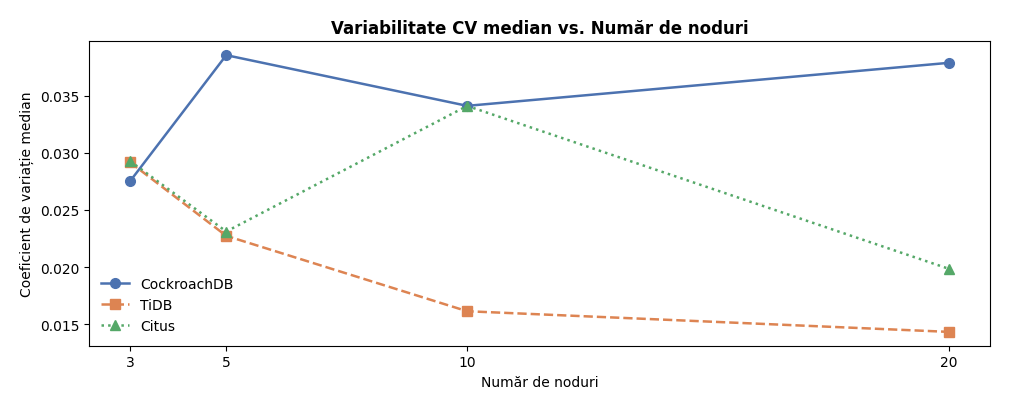
\includegraphics[width=\textwidth]{fig/global_cv_vs_nodes.png}
    \caption{Coeficientul de variație median al rulărilor temporizate, agregat pe toate interogările executabile, în funcție de numărul de noduri.}
    \label{fig:global_cv_vs_nodes}
\end{figure}

Stabilitatea măsurătorilor între rulări, prezentată în figura \ref{fig:global_cv_vs_nodes} prin coeficientul de variație agregat, oferă o perspectivă complementară. TiDB prezintă cea mai mare stabilitate, cu un coeficient de variație care descrește monoton de la $0,029$ la 3 noduri până la $0,014$ la 20 de noduri. Citus prezintă un comportament mai zgomotos dar care se stabilizează la configurațiile mari (CV de $0,020$ la 20 de noduri). CockroachDB rămâne sistemul cu cea mai mare variabilitate, oscilând în jurul valorii de $0,038$.

\begin{table}[H]
\centering
\begin{tabular}{lllll}
\multicolumn{1}{c}{Bază de date} & \multicolumn{1}{c}{media} & median & min  & max   \\
Citus                            & 5,93                      & 5,22   & 0,90 & 18,63 \\
CockroachDB                      & 3,33                      & 3,16   & 0,42 & 6,05  \\
TiDB                             & 1,34                      & 1,07   & 0,76 & 3,23 
\end{tabular}
\caption{Sumar accelerație relativă la linia de bază cu 3 noduri}
\end{table}